%%%%%%%%%%%%%%%%%%%%%%%%%%%%%%%%%%%%%%%%%
% Tufte-Style Book (Documentation Template)
% LaTeX Template
% Version 1.0 (5/1/13)
%
% This template has been downloaded from:
% http://www.LaTeXTemplates.com
%
% Original author:
% The Tufte-LaTeX Developers (tufte-latex.googlecode.com)
%
% License:
% Apache License (Version 2.0)
%
% IMPORTANT NOTE:
% In addition to running BibTeX to compile the reference list from the .bib
% file, you will need to run MakeIndex to compile the index at the end of the
% document.
%
%%%%%%%%%%%%%%%%%%%%%%%%%%%%%%%%%%%%%%%%%

%--------------------------------------------------------------------------
%	PACKAGES AND OTHER DOCUMENT CONFIGURATIONS
%------------------------------------------------------------------------

\documentclass[oneside,openany]{tufte-book} % Use the tufte-book class which in turn uses the tufte-common class

\hypersetup{colorlinks} % Comment this line if you don't wish to have colored links
\usepackage{hyperref}
\usepackage{microtype} % Improves character and word spacing
\usepackage[utf8]{inputenc}
\usepackage{listings}
\usepackage{lipsum} % Inserts dummy text
\usepackage{booktabs} % Better horizontal rules in tables
\usepackage{graphicx} % Needed to insert images into the document
\graphicspath{{graphics/}} % Sets the default location of pictures
\setkeys{Gin}{width=\linewidth,totalheight=\textheight,keepaspectratio} % Improves figure scaling
\usepackage{tikz}
\usetikzlibrary{patterns}
\usepackage{fancyvrb} % Allows customization of verbatim environments
\fvset{fontsize=\normalsize} % The font size of all verbatim text can be changed here

\newcommand{\hangp}[1]{\makebox[0pt][r]{(}#1\makebox[0pt][l]{)}} % New command to create parentheses around text in tables which take up no horizontal space - this improves column spacing
\newcommand{\hangstar}{\makebox[0pt][l]{*}} % New command to create asterisks in tables which take up no horizontal space - this improves column spacing

\usepackage{xspace} % Used for printing a trailing space better than using a tilde (~) using the \xspace command

\newcommand{\monthyear}{\ifcase\month\or January\or February\or March\or April\or May\or June\or July\or August\or September\or October\or November\or December\fi\space\number\year} % A command to print the current month and year

\newcommand{\openepigraph}[2]{ % This block sets up a command for printing an epigraph with 2 arguments - the quote and the author
\begin{fullwidth}
\sffamily\large
\begin{doublespace}
\noindent\allcaps{#1}\\ % The quote
\noindent\allcaps{#2} % The author
\end{doublespace}
\end{fullwidth}
}

\newcommand{\blankpage}{\newpage\hbox{}\thispagestyle{empty}\newpage} % Command to insert a blank page

\usepackage{units} % Used for printing standard units
\usepackage[shortlabels]{enumitem}

\newcommand{\hlred}[1]{\textcolor{Maroon}{#1}} % Print text in maroon
\newcommand{\hangleft}[1]{\makebox[0pt][r]{#1}} % Used for printing commands in the index, moves the slash left so the command name aligns with the rest of the text in the index 
\newcommand{\hairsp}{\hspace{1pt}} % Command to print a very short space
\newcommand{\ie}{\textit{i.\hairsp{}e.}\xspace} % Command to print i.e.
\newcommand{\eg}{\textit{e.\hairsp{}g.}\xspace} % Command to print e.g.
\newcommand{\na}{\quad--} % Used in tables for N/A cells
\newcommand{\measure}[3]{#1/#2$\times$\unit[#3]{pc}} % Typesets the font size, leading, and measure in the form of: 10/12x26 pc.
\newcommand{\tuftebs}{\symbol{'134}} % Command to print a backslash in tt type in OT1/T1

\providecommand{\XeLaTeX}{X\lower.5ex\hbox{\kern-0.15em\reflectbox{E}}\kern-0.1em\LaTeX}
\newcommand{\tXeLaTeX}{\XeLaTeX\index{XeLaTeX@\protect\XeLaTeX}} % Command to print the XeLaTeX logo while simultaneously adding the position to the index

\newcommand{\doccmdnoindex}[2][]{\texttt{\tuftebs#2}} % Command to print a command in texttt with a backslash of tt type without inserting the command into the index

\newcommand{\doccmddef}[2][]{\hlred{\texttt{\tuftebs#2}}\label{cmd:#2}\ifthenelse{\isempty{#1}} % Command to define a command in red and add it to the index
{ % If no package is specified, add the command to the index
\index{#2 command@\protect\hangleft{\texttt{\tuftebs}}\texttt{#2}}% Command name
}
{ % If a package is also specified as a second argument, add the command and package to the index
\index{#2 command@\protect\hangleft{\texttt{\tuftebs}}\texttt{#2} (\texttt{#1} package)}% Command name
\index{#1 package@\texttt{#1} package}\index{packages!#1@\texttt{#1}}% Package name
}}

\newcommand{\doccmd}[2][]{% Command to define a command and add it to the index
\texttt{\tuftebs#2}%
\ifthenelse{\isempty{#1}}% If no package is specified, add the command to the index
{%
\index{#2 command@\protect\hangleft{\texttt{\tuftebs}}\texttt{#2}}% Command name
}
{%
\index{#2 command@\protect\hangleft{\texttt{\tuftebs}}\texttt{#2} (\texttt{#1} package)}% Command name
\index{#1 package@\texttt{#1} package}\index{packages!#1@\texttt{#1}}% Package name
}}

% A bunch of new commands to print commands, arguments, environments, classes, etc within the text using the correct formatting
\newcommand{\docopt}[1]{\ensuremath{\langle}\textrm{\textit{#1}}\ensuremath{\rangle}}
\newcommand{\docarg}[1]{\textrm{\textit{#1}}}
\newenvironment{docspec}{\begin{quotation}\ttfamily\parskip0pt\parindent0pt\ignorespaces}{\end{quotation}}
\newcommand{\docenv}[1]{\texttt{#1}\index{#1 environment@\texttt{#1} environment}\index{environments!#1@\texttt{#1}}}
\newcommand{\docenvdef}[1]{\hlred{\texttt{#1}}\label{env:#1}\index{#1 environment@\texttt{#1} environment}\index{environments!#1@\texttt{#1}}}
\newcommand{\docpkg}[1]{\texttt{#1}\index{#1 package@\texttt{#1} package}\index{packages!#1@\texttt{#1}}}
\newcommand{\doccls}[1]{\texttt{#1}}
\newcommand{\docclsopt}[1]{\texttt{#1}\index{#1 class option@\texttt{#1} class option}\index{class options!#1@\texttt{#1}}}
\newcommand{\docclsoptdef}[1]{\hlred{\texttt{#1}}\label{clsopt:#1}\index{#1 class option@\texttt{#1} class option}\index{class options!#1@\texttt{#1}}}
\newcommand{\docmsg}[2]{\bigskip\begin{fullwidth}\noindent\ttfamily#1\end{fullwidth}\medskip\par\noindent#2}
\newcommand{\docfilehook}[2]{\texttt{#1}\index{file hooks!#2}\index{#1@\texttt{#1}}}
\newcommand{\doccounter}[1]{\texttt{#1}\index{#1 counter@\texttt{#1} counter}}
\usepackage{pst-node}
\usepackage{makeidx} % Used to generate the index
\makeindex % Generate the index which is printed at the end of the document

% This block contains a number of shortcuts used throughout the book
\newcommand{\vdqi}{\textit{VDQI}\xspace}
\newcommand{\pfds}{\textbf{\textit{PFDS}}\xspace}
\newcommand{\fp}{\textbf{\textit{FP}}\xspace}
\newcommand{\ds}{\textbf{\textit{DS}}\xspace}
\newcommand{\sh}{\textbf{\textit{WFSM}}\xspace}
\newcommand{\ei}{\textit{EI}\xspace}
\newcommand{\ve}{\textit{VE}\xspace}
\newcommand{\be}{\textit{BE}\xspace}
\newcommand{\VDQI}{\textit{The Visual Display of Quantitative Information}\xspace}
\newcommand{\EI}{\textit{Envisioning Information}\xspace}
\newcommand{\VE}{\textit{Visual Explanations}\xspace}
\newcommand{\BE}{\textit{Beautiful Evidence}\xspace}
\newcommand{\TL}{Tufte-\LaTeX\xspace}

\definecolor{punct}{rgb}{0.0,0.24313725490196078,1.0}
\definecolor{numb}{rgb}{0.0,0.24313725490196078,1.0}
\usepackage[svgnames]{xcolor} % Enabling colors by their 'svgnames'
%----------------------------------------------------------------------------------------
%	BOOK META-INFORMATION
%----------------------------------------------------------------------------------------

\title{Characterization of topological models for distributed computing with logical systems.} % Title of the book

\author{Fabián Romero } % Author

\publisher{
  A thesis submitted in partial fulfillment \\
  of the requirements for the degree of\\
  Master of Computer Sciences \\
  University of Mexico (UNAM)

  Posgrado en Ciencia e Ingeniería de la Computación\\
Supervisor: Francisco Hernández Quiroz} % Publisher

%----------------------------------------------------------------------------------------

\begin{document}
\lstdefinelanguage{json}{
    basicstyle=\normalfont\ttfamily,
    numbers=left,
    framexleftmargin=0pt,
    xleftmargin=2em,
    numberstyle=\scriptsize,
    stepnumber=1,
    numbersep=8pt,
    showstringspaces=false,
    breaklines=true,
    morecomment=[s]{/*}{*/},
    morecomment=[l]--,
    frame=lines,
%    backgroundcolor=\color{background},
    literate=
     *{0}{{{\color{numb}0}}}{1}
      {1}{{{\color{numb}1}}}{1}
      {2}{{{\color{numb}2}}}{1}
      {3}{{{\color{numb}3}}}{1}
      {4}{{{\color{numb}4}}}{1}
      {5}{{{\color{numb}5}}}{1}
      {6}{{{\color{numb}6}}}{1}
      {7}{{{\color{numb}7}}}{1}
      {8}{{{\color{numb}8}}}{1}
      {9}{{{\color{numb}9}}}{1}
      {:}{{{\color{punct}{:}}}}{1}
      {,}{{{\color{punct}{,}}}}{1}
      {\{}{{{\color{delim}{\{}}}}{1}
      {\}}{{{\color{delim}{\}}}}}{1}
      {[}{{{\color{delim}{[}}}}{1}
      {]}{{{\color{delim}{]}}}}{1},
}
\maketitle % Print the title page

%----------------------------------------------------------------------------------------
%	COPYRIGHT PAGE
%----------------------------------------------------------------------------------------
\newpage
\begin{fullwidth}
~\vfill
\thispagestyle{empty}
\setlength{\parindent}{0pt}
\setlength{\parskip}{\baselineskip}
Copyright \copyright\ \the\year\ \thanklessauthor

\par\smallcaps{Published by \thanklesspublisher}

\par\smallcaps{tufte-latex.googlecode.com}

\par Licensed under the Apache License, Version 2.0 (the ``License''); you may not use this file except in compliance with the License. You may obtain a copy of the License at \url{http://www.apache.org/licenses/LICENSE-2.0}. Unless required by applicable law or agreed to in writing, software distributed under the License is distributed on an \smallcaps{``AS IS'' BASIS, WITHOUT WARRANTIES OR CONDITIONS OF ANY KIND}, either express or implied. See the License for the specific language governing permissions and limitations under the License.\index{license}

\end{fullwidth} 

%----------------------------------------------------------------------------------------
\tableofcontents % Print the table of contents

%----------------------------------------------------------------------------------------
%	INTRODUCTION
%----------------------------------------------------------------------------------------
\chapter{Abstract}


The objective of this work is to study the topological model for distributed computing from a formal logic perspective by mapping those topological models to Kripke frames and then study then by applying model checking and other techniques. Specifically targeting consensus problem as a subject of study.

\chapter{Introduction} 

Today, large data processing facilities provide significant computing capabilities. Being able to orchestrate them in a coherent way will unleash enourmus computing power currently underutilized. In order to do so, we need more comprehensive models for \ds. There are new and exiting methods which allow to study \ds which provide new ways to explore them theoretically and even create effectively computations to find relevant properties.\\

A distributed system \ds can be defined operationally as a collection of processes executing a protocol (algorithm) within a communicating environment.

Studying \ds operationally has shown to be a complex task, even when the number of processes and connections is limited and/or following simple patterns. 
It's complexity arises from the number of possible interactions between their 
elements and the dynamics of such interactions.\\

For example, internet services are higly complex environments containing hundreds, thousands or even millions of components, all of them interacting, the events of the communications and changes of state yields a combinatorial explosion.

On it's seminal paper \cite{Herlihy1999} Herlihy  introduced a characterization of \ds, 
mapping the specifics of such protocols and environments to a topological structure.
In this combinatorial description all possible events on the of the interactions dynamics  are represented {\bf simultaneously} on a single topological structure.\\
Such approach is a deliberated trade off. Interchanging one model with complex 
dynamics for other with far more elements in a complex entanglement. But quite importantly, this model is static.\\

This technique for the analysis of \ds has gained significant traction 
and has become widely used.
Gaining from a large set of topology results that can be immediately applied, and, as 
he argues. Our minds are much better equipped for analyzing static entities even when they are very complex than for dynamic ones even if they are sparse.

\ds have been studied from many areas and multiple angles, in particular, it has been 
covered on many different logic approaches, epistemic logic \cite{Meyer:1995} is a natural formulation for them, there's a great tradition on the field of artificial intelligence associating several logics to the study of \ds \cite{HandbookAI1}, and many other logics as multi modal logic \cite{Hintikka1962}, dynamic epistemic logic \cite{Ditmarsch:2007}, among many others.

Those works are intended to comprehend communications, epistemic development and behavior of such systems from an operational point of view.\\

This work has a different intention, the main idea is to preserve the spirit of Herlihy's work by creating a large static structure representing all possible states and transitions 



\chapter{General Objective}

The objective of this work, is to mimic the approach taken by Herlihy but using formal logic as model, first, by mapping topological descriptions of {\ds} into Kripke frames. Then, by studying a specific problem in the light of logical systems. The problem to study will be the consensus problem on the wait free shared memory model (\sh).

\chapter{Specific Objectives}


\begin{itemize}[topsep=0pt,itemsep=-1ex,partopsep=1ex,parsep=1ex]
\item Describe a way to map topological models to Kripke frames.
\item Study which properties such frames will have.
\end{itemize}

%

%Ever since Herlihy  introduced it. The topological characterization for distributed computing has gained significant traction. And has become a widely used technique for the analysis of distributed systems. In which, a distributed system is regarded as a collection of processes executing a protocol within a communicating environment. Mapping the specifics of such processes and their environment to a topological structure.\\

%Such view it is completely compatible with the studies of many logical systems. For example, epistemic logic is a natural formulation of it. Many other logical systems map the assumptions of knowledge of communicating agents. Such as multi modal logic, dynamic logic etc.

%The goal of this project is to propose a formal logical system which can model a topological characterization of DC. And to map every axiom, inference rule and formula to a topological structure. ?

%The goal of this project is to propose a tolerant sequence of formal theories for which a topological characterization of DC can be a model. ?

%How we express the weakness of  logic

\chapter{Background} % The asterisk leaves out this chapter from the table of contents
\section{Distributed computing, wait free shared memory model \sh}

Very early on the study of distributed systems, Leslie Lamport noticed an important trait of them: There is a partial order on the set of all system events. \cite{Lamport78}. He also show how to find a total order for a specific model, but this is not limited to such model, the {\bf order-extension principle} states that a total order can be found as a linear extension for any partial order.\\

Lets consider $n$ identified processes communicating in a shared memory environment running a wait-free protocol. Such as that described on \cite{Herlihy1999}.\\

\begin{lstlisting}[mathescape,language=json,firstnumber=1,basicstyle=\footnotesize,commentstyle=\color{gray},caption={Normal form wait free protocol},label=amb]
--code for process i 
update(i,a,input_value)    -- a[i] := input_value
for round in 1 .. r do
   local_state:=scan(a)
   update(i,a,local_state) -- a[i] := local_state
return $\displaystyle \delta $(local_state)
\end{lstlisting}

So, the partial order induced by such algorithm, says if $a \ge b$ in time, meaning $b$ updated the shared memory not latter than $a$, also can be interpreted as $a$ ``knows'' the state of $b$. \\
Observe that this simple fact will have a deep impact when we translate this model to a logic system, because it means we can derive epistemic results from the adequate accessibility semantics.\\
It is easy to find a total order in this case, as the time (in the clock of the shared memory) when writings were done.

\subsection{Partial Orders}

{\bf Definitions}
\begin{itemize}
\item[{\bf poset}] A partially ordered set (a.k.a poset) is a pair $(P,\ge)$ where $P$ is a finite set and $\ge$ is a reflexive, anti symmetric and transitive relation over $P$.
\item[{\bf linear extension}] Given a poset $(P,\ge)$ let $\lambda$ be a bijection from $P$ to $\{1,...,|P|\}$ such that $\forall i,j$ if $|P| \ge j > i \ge 1$ then $\lambda(j) > \lambda(i)$. $\lambda$ is a linear extension
\item[{\bf order polytope}] The following linear constraints:\\
$$
O(P)=\{X\in \mathbb{R}^{|P|} | 1 \ge X_i \ge 0, X_i > X_j \quad if \quad x_i > x_j \quad in \quad P  \}
$$

Define a polytope $O(P)$ in $ \mathbb{R}^{|P|} $, such polytope is called order polytope of  $P$ \cite{Stanley1986}
\end{itemize}

{\bf Theorem} The number of distinct linear extensions of the poset $(P,\ge)$ equals the number of simplices in a maximal size triangulation of the order polytope $O(P)$ \\

\section{The Topological Structure of Asynchronous Computability}

Once we have established that fact, if we consider all possible orderings of events under \sh, we know by symmetry that they are manifolds.\\

The interpretation is the following:\\
Every element of $P$ is a process, every simplex where it is contained is the {\bf linear extension} of all process contained on that simplex.

Let see for example, the case of 3 processes and a single round of communication.\\


All total orders (possible executions):

\begin{tabular}{ l | r r r r}
  \hline                       
$ order$ & $=,=$ & $=,<$ & $<,=$ & $<,<$\\
  \hline                       
$a b c$ & $a=b=c$ & $a=b<c$ & $a<b=c$ & $a<b<c$\\
$a c b$ &         & $a=c<b$ &         & $a<c<b$\\
$b a c$ &         &         & $b<a=c$ & $b<a<c$\\
$b c a$ &         & $b=c<a$ &         & $b<c<a$\\
$c a b$ &         &         & $c<a=b$ & $c<a<b$\\
$c b a$ &         &         &         & $c<b<a$\\
  \hline  
\end{tabular}

Those are all (13) possible executions, in this model, they will be faces.\\
A node, can view all elements that are lesser or equals than itself, and only knows that.

So, all nodes are:
\begin{tabular}{ c}
  \hline                       
$a$ \\
$a \le b$ \\
$b \le a$ \\
$b$ \\
$b \le c$ \\
$c \le b$ \\
$c$ \\
$c \le a$ \\
$a \le c$ \\
$ {a,b} \le c$ \\
$ {b,c} \le a$ \\
$ {c,a} \le b$ \\
  \hline  
\end{tabular}


And the simplicial complex will be:

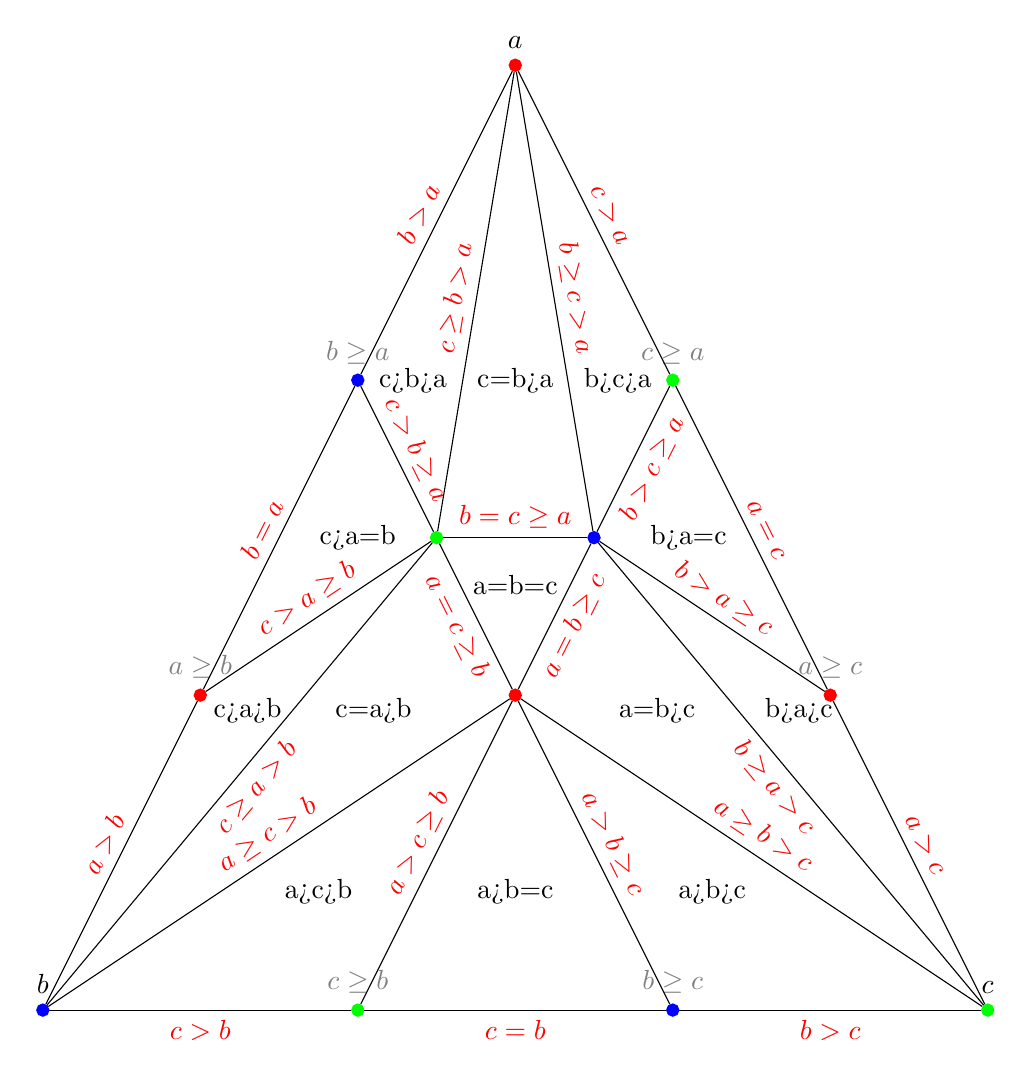
\begin{tikzpicture}
    \tikzstyle{red}=[circle,thick,draw=red,fill=red,inner sep=0pt,minimum width=4pt,minimum height=4pt]
    \tikzstyle{blue}=[circle,thick,draw=blue,fill=blue,inner sep=0pt,minimum width=4pt,minimum height=4pt]
    \tikzstyle{green}=[circle,thick,draw=green,fill=green,inner sep=0pt,minimum width=4pt,minimum height=4pt]
    \tikzstyle{point}=[circle,thick,draw=black,fill=black,inner sep=0pt,minimum width=4pt,minimum height=4pt]
    \node (a)[red,label={$a$}]     at (6,12) {};
    \node (b)[blue,label={$b$}]    at (0,0) {};
    \node (c)[green,label={$c$}]   at (12,0) {};
    \node (ab)[red,label={{\color{gray}$a \ge b $}}]    at (2,4) {};
    \node (ba)[blue,label={{\color{gray}$b \ge a $}}]   at (4,8) {};
    \node (ca)[green,label={{\color{gray}$c \ge a $}}]  at (8,8) {};
    \node (ac)[red,label={{\color{gray}$a \ge c $}}]    at (10,4) {};
    \node (cb)[green,label={{\color{gray}$c \ge b $}}]  at (4,0) {};
    \node (bc)[blue,label={{\color{gray}$b \ge c $}}]   at (8,0) {};

    \node (cba)[green] at (5,6) {};
    \node (bca)[blue]  at (7,6) {};
    \node (abc)[red]   at (6,4) {};
    \draw (a)   -- (ba)   node[pos=0.5,sloped,above] {{\color{red}$b>a$}};
    \draw (ba)  -- (ab)   node[pos=0.5,sloped,above] {{\color{red}$b=a$}};
    \draw (ab)  -- (b)    node[pos=0.5,sloped,above] {{\color{red}$a>b$}};
    \draw (b)   -- (cb)   node[pos=0.5,sloped,below] {{\color{red}$c>b$}};
    \draw (cb)  -- (bc)   node[pos=0.5,sloped,below] {{\color{red}$c=b$}};
    \draw (bc)  -- (c)    node[pos=0.5,sloped,below] {{\color{red}$b>c$}};
    \draw (c)   -- (ac)   node[pos=0.5,sloped,above] {{\color{red}$a>c$}};
    \draw (ac)  -- (ca)   node[pos=0.5,sloped,above] {{\color{red}$a=c$}};
    \draw (ca)  -- (a)    node[pos=0.5,sloped,above] {{\color{red}$c>a$}};
    \draw (ba)  -- (cba)  node[pos=0.5,sloped,above] {{\color{red}$c > b \ge a$}};
    \draw (ab)  -- (cba)  node[pos=0.5,sloped,above] {{\color{red}$c > a \ge b$}};
    \draw (cb)  -- (abc)  node[pos=0.5,sloped,above] {{\color{red}$a > c \ge b$}};
    \draw (bc)  -- (abc)  node[pos=0.5,sloped,above] {{\color{red}$a > b \ge c$}};
    \draw (ac)  -- (bca)  node[pos=0.5,sloped,above] {{\color{red}$b > a \ge c$}};
    \draw (ca)  -- (bca)  node[pos=0.5,sloped,below] {{\color{red}$b > c \ge a$}};
    \draw (a)   -- (cba)  node[pos=0.5,sloped,above] {{\color{red}$c \ge b > a$}};
    \draw (a)   -- (bca)  node[pos=0.5,sloped,above] {{\color{red}$b \ge c > a$}};
    \draw (b)   -- (cba)  node[pos=0.5,sloped,below] {{\color{red}$c \ge a > b$}};
    \draw (b)   -- (abc)  node[pos=0.5,sloped,above] {{\color{red}$a \ge c > b$}};
    \draw (c)   -- (abc)  node[pos=0.5,sloped,above] {{\color{red}$a \ge b > c$}};
    \draw (c)   -- (bca)  node[pos=0.5,sloped,below] {{\color{red}$b \ge a > c$}};
    \draw (cba) -- (bca)  node[pos=0.5,sloped,above] {{\color{red}$b = c \ge a$}};
    \draw (bca) -- (abc)  node[pos=0.5,sloped,below] {{\color{red}$a = b \ge c$}};
    \draw (abc) -- (cba)  node[pos=0.5,sloped,below] {{\color{red}$a = c \ge b$}};
    \node at (3.5,1.5) {a>c>b};
    \node at (6,1.5) {a>b=c};
    \node at (8.5,1.5) {a>b>c};
    \node at (2.6,3.8) {c>a>b};
    \node at (4.2,3.8) {c=a>b};
    \node at (6.0,5.4) {a=b=c};
    \node at (7.8,3.8) {a=b>c};
    \node at (9.6,3.8) {b>a>c};
    \node at (4.0,6.0) {c>a=b};
    \node at (8.2,6.0) {b>a=c};
    \node at (4.7,8.0) {c>b>a};
    \node at (6.0,8.0) {c=b>a};
    \node at (7.3,8.0) {b>c>a};
\end{tikzpicture}\\
\newpage
Remarks
\begin{itemize}[topsep=0pt,itemsep=-1ex,partopsep=1ex,parsep=1ex]
\item Every face (triangle) is a possible execution (total order).
\item Given the edges of a triangle, the execution is the linear extension of them.
\item Two triangles joined by an edge are two executions where 2 processes can't distinguish between (those are the processes in the edge).
\item Any edge belonging to two triangles has exactly one $\le$ sign.
\item If two triangles are joined by an edge, their execution is one the case ``='' and the other ``>'' in the $\le$ sign.
\item two triangles are joined by only a vertex, are such that only that process can't distinguish between them.
\end{itemize}


\section{Kripke structures}

\section{Definition}

A multi modal Kripke structure is a pair $K = (W, \rightarrow)$ where $W$ is a set of worlds and $\rightarrow$ is a family of relations $\rightarrow_i \subseteq W \times W$ indexed by a fixed set $I$.\\

A multi modal Kripke model is a tuple $M=(W,\rightarrow,P,V)$ where $(W, \rightarrow)$ is a Kripke structure, $P$ is the set of propositional constants, and $V:W\rightarrow \mathcal{P}(P)$ is a valuation function\\

A formula in $\mathcal{L}(P)$ is interpreted in a Kripke model \\
$M=(W,\rightarrow,P,V)$ at some $w\in W$ as follows:
\begin{itemize}[topsep=0pt,itemsep=-1ex,partopsep=1ex,parsep=1ex]
\item $(M,w) \models p$ iff $p\in V(w)$
\item $(M,w) \models \ \phi_1 \vee \phi_2$ iff $(M,w) \models \ \phi_1$ or $(M,w) \models \ \phi_2$
\item $(M,w) \models \ \neg\phi$ if is not the case that $(M,w) \models \phi$
\item $(M,w) \models \ \langle i \rangle \phi$ iff there exists $w'\in W$ such that:\\ $w\rightarrow_i w'$ and  $(M,w') \models \ \phi$
\end{itemize}

We will use the total order as  propositional constants, for the example we are dealing with, possible executions are here $W$, let's see accesibility for agent $a$ 

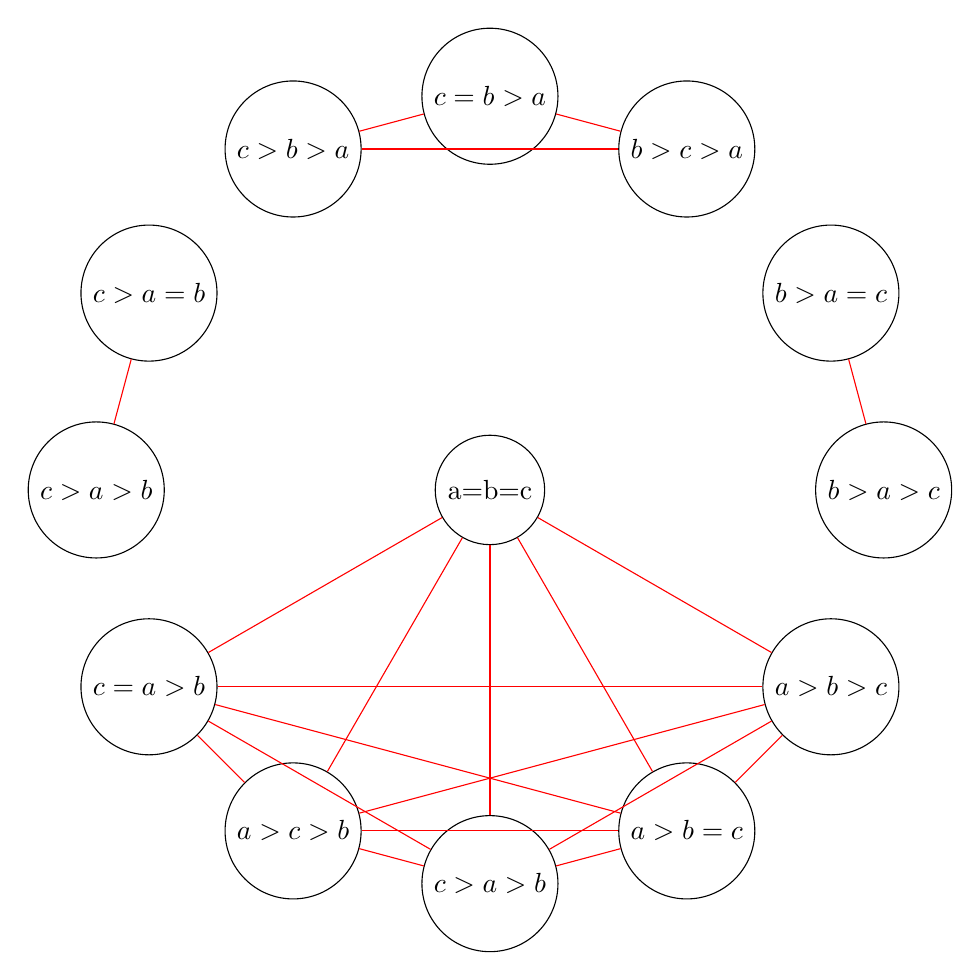
\begin{tikzpicture}
\node (c)[circle,draw] at (0,0) {a=b=c};
\foreach \angle/\label in {0/{$b>a>c$},30/{$b>a=c$},60/{$b>c>a$},90/{$c=b>a$},120/{$c>b>a$},150/{$c>a=b$},180/{$c>a>b$},210/{$c=a>b$},240/{$a>c>b$},270/{$c>a>b$},300/{$a>b=c$},330/{$a>b>c$}}
\node[circle,draw] (\angle) at (\angle:5) {\label};
\foreach \node/\to in {210/240,210/270,210/300,210/330,240/300,240/330,270/330,60/90,90/120,120/60,0/30,150/180,240/270,270/300,300/330}
\draw[red] (\node)  -- (\to)node {};%[pos=0.5,sloped,above];// {{\color{red}$a$}};
\foreach \node in {210,240,...,330}
\draw[red] (c)  -- (\node)node {};%[pos=0.5,sloped,above] {{\color{red}$a$}};
\end{tikzpicture}

We can see all three agents simultaneously:\\

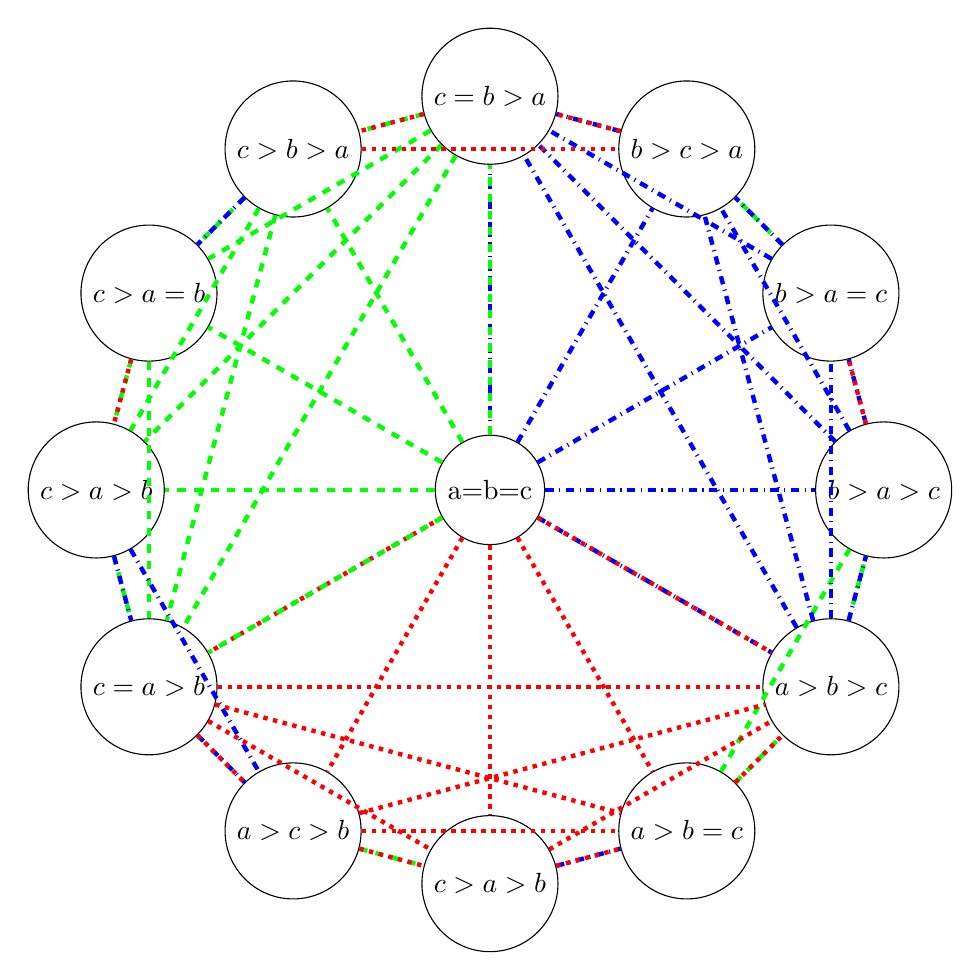
\begin{tikzpicture}
\node (c)[circle,draw] at (0,0) {a=b=c};
\foreach \angle/\label in {0/{$b>a>c$},30/{$b>a=c$},60/{$b>c>a$},90/{$c=b>a$},120/{$c>b>a$},150/{$c>a=b$},180/{$c>a>b$},210/{$c=a>b$},240/{$a>c>b$},270/{$c>a>b$},300/{$a>b=c$},330/{$a>b>c$}}
\node[circle,draw] (\angle) at (\angle:5) {\label};
\foreach \node/\to in {90/120,90/150,90/180,90/210,120/150,120/180,120/210,150/180,150/210,180/210,300/330,330/0,300/0,30/60,240/270}
\draw[green,dashed,ultra thick] (\node)  to  (\to)node {};%[pos=0.5,sloped,above];// {{\color{red}$a$}};
\foreach \node/\to in {330/0,330/30,330/60,330/90,0/30,0/60,0/90,30/60,30/90,60/90,180/210,180/240,210/240,120/150,270/300}
\draw[blue,dashdotted,ultra thick] (\node)  to  (\to)node {};%[pos=0.5,sloped,above];// {{\color{red}$a$}};
\foreach \node/\to in {210/240,210/270,210/300,210/330,240/300,240/330,270/330,60/90,90/120,120/60,0/30,150/180,240/270,270/300,300/330}
\draw[red,dotted,ultra thick] (\node)  -- (\to)node {};%[pos=0.5,sloped,above];// {{\color{red}$a$}};
\foreach \node in {330,0,30,60,90}
\draw[blue,dashdotted,ultra thick] (c)  -- (\node)node {};%[pos=0.5,sloped,above] {{\color{red}$a$}};
\foreach \node in {210,240,...,330}
\draw[red,dotted,ultra thick] (c)  -- (\node)node {};%[pos=0.5,sloped,above] {{\color{red}$a$}};
\foreach \node in {90,120,...,210}
\draw[green,dashed,ultra thick] (c)  -- (\node)node {};%[pos=0.5,sloped,above] {{\color{red}$a$}};
\end{tikzpicture}


\subsection{Remarks}

\begin{itemize}[topsep=0pt,itemsep=-1ex,partopsep=1ex,parsep=1ex]
\item transitivity.
\item reflexivity.
\item every world has access to another world for every modality.
\end{itemize}


%----------------------------------------------------------------------------------------

\backmatter

%----------------------------------------------------------------------------------------
%	BIBLIOGRAPHY
%----------------------------------------------------------------------------------------

\bibliography{bibliography} % Use the bibliography.bib file for the bibliography
\bibliographystyle{plainnat} % Use the plainnat style of referencing

%----------------------------------------------------------------------------------------

%\printindex % Print the index at the very end of the document

\end{document}
